\PageHeading{09}{案例B · 职场办公公众号}{同一款产品，围绕差旅、外设与工作任务重排内容}
\ModeLocal
\begin{note}\small
\Lead{任务}\quad HUAWEI MateBook 14（鸿蒙版）／经常出差的移动办公者／职场办公／对比选择／到店体验／公众号。\par
\Lead{实际结果}\quad 已确认大纲v1，内联样式文章HTML及1200$\times$900封面；本轮实际运行，未调用模型或ima。
\end{note}
\begin{minipage}[t]{.49\linewidth}\vspace{0pt}
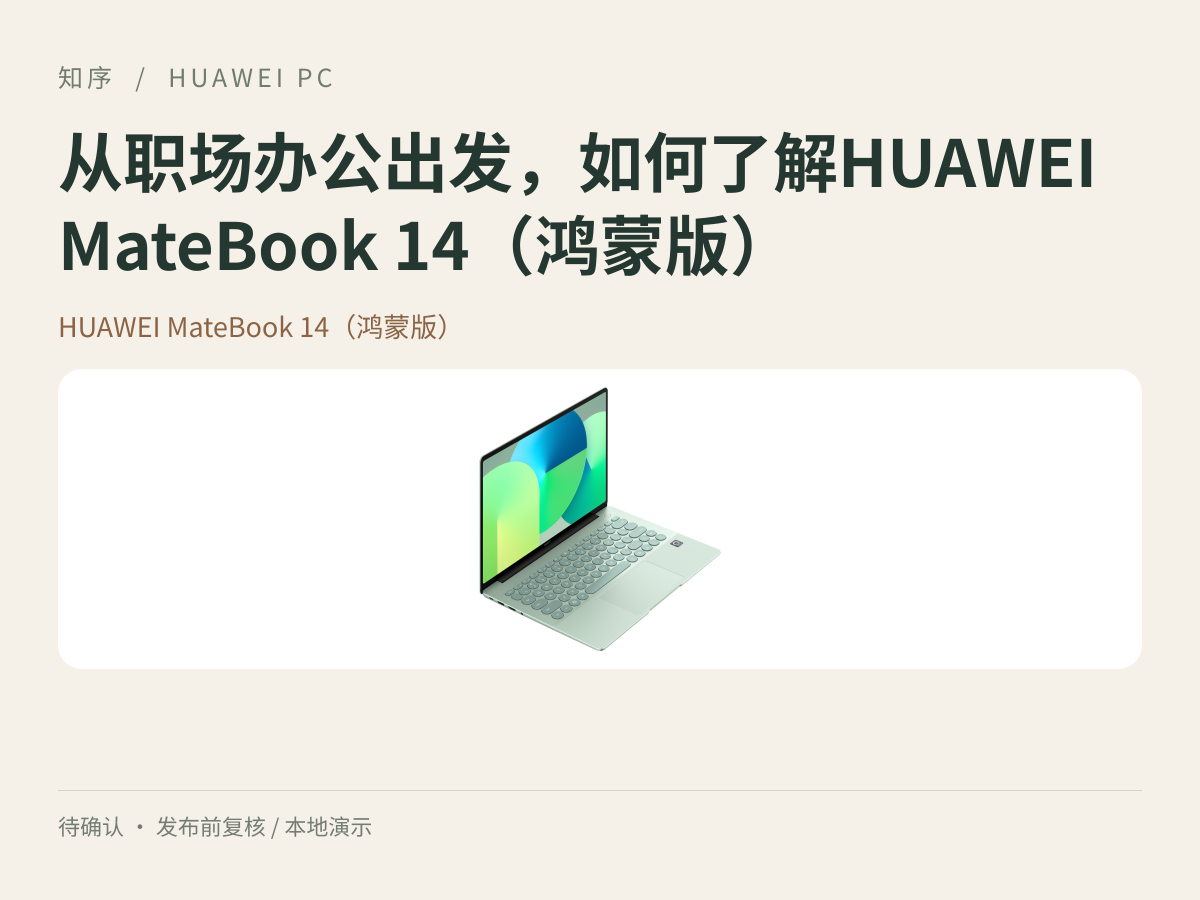
\includegraphics[width=\linewidth]{case-b-1.png}
\ImgCap{实际生成的公众号封面；完整文章HTML随说明书源项目中的evidence目录交付。}
\end{minipage}\hfill
\begin{minipage}[t]{.47\linewidth}\vspace{0pt}
\Lead{结构如何变化}\par
1. 先说明差旅办公的选型问题；\par
2. 解释携带与外设连接条件；\par
3. 提醒额定电池容量的口径；\par
4. 用软件、外设与文件任务清单收束；\par
5. 邀请到店核对对应销售版本。

\Lead{与案例A的区别}\par
以分段解释和决策核对代替收藏型短笔记；图片数量按公众号2--4张约束，行动引导转向携带工作任务到店沟通。
\end{minipage}
\Sub{实际生成内容节选}
\begin{excerpt}\small
\Lead{\CaseBTitle}\par
\CaseBIntro\par\vspace{1mm}
\Lead{把参数放回使用流程}\par
\CaseBLast
\end{excerpt}
\Lead{事实表达的边界}\quad 接口与电池信息只作为核对维度，不由接口存在推导所有外设都兼容，不承诺未经资料支持的应用适配、远程管理政策或续航表现。

\Lead{来源与审核}\quad 使用同型号本地产品事实和图片索引，实际审核为needs\_attention。本文选录属于规则演示；可证明不同场景下的组织变化，不能替代模型语言质量评估或ima正式来源核验。
\SourceNote{本轮实际生成，evidence/case-b.json及case-b-wechat.html。}
